%% Sect. 5 -- from augur_AMT_§5 draft v6 (2026-09-22); condensed 2026-09-29. The four "What the pipeline could
%% report instead" blocks are folded into single sentences pointing to Sect. 6.1.
\section{What the pipeline already knows and does not report}
\label{sec:5}

Section~\ref{sec:4} measured errors that leave no trace in the residual. This section concerns the second category:
information that already exists in the pipeline -- in the profiled objective, the optimiser's termination state,
the knot table and the timestamps of the files being read -- and is discarded before the product is written.
Reporting it requires neither a better algorithm nor an additional measurement.

\subsection{A nonlinear parameter the data do not determine}
\label{sec:5.1}

A converged nonlinear fit has established only that it sits at a stationary point of the profiled residual. If the
profiled residual is nearly flat over the range the parameter may take, the returned value is set by the starting
point and the bounds, and the uncertainty computed from the local curvature describes a curvature that is not there. Standard DOAS software reports the parameter value without reporting how much the data
constrain it. We test this on the wavelength shift, the parameter least distinguishable from a change in the background. The shift is
scanned across $\pm 4$\,px with the linear parameters profiled out at each point, a profile-likelihood analysis of
practical identifiability in the sense of \citet{Raue_2009}.

In the cold channel the objective is flat. For twelve ambient spectra the ratio of the largest to the smallest
profiled residual sum of squares has a median of \fieldnum{1.0120} and never exceeds \fieldnum{1.0611}. In a larger set of \fieldnum{165}
spectra the minimum lies at an edge of the scanned range in \fieldnum{77}\,\% of cases, and evaluating the objective at zero
shift rather than at its minimum costs \fieldnum{0.01}\,\% to \fieldnum{4.35}\,\%. The same scan in the hot PNs channel spans
a factor of $\fieldnum{3.09\times10^{5}}$. Two implementations confirm that the consequence is not numerical. Under matched
settings the shift returned for the same spectra is \fieldnum{$-2.014$}\,px in this work, with \fieldnum{85.5}\,\% of fits terminating
at a bound, against \fieldnum{$-0.088$}\,px from QDOAS with \fieldnum{4.5}\,\% at a bound; tightening the QDOAS convergence threshold to
$10^{-12}$ changes nothing. Both codes converge and report values two pixels apart, because the data do not
distinguish them.

The same channel locates the shift when the absorber is strong enough. On 2 June NO$_2$ from a cylinder standard
(nominally 10\,$\mu$mol\,mol$^{-1}$ in N$_2$, past its certification date and used here only for its spectrum) was added
to zero air in the cold cavity for half an hour. Retrieved against the preceding zero-air spectrum with the
operational reference and window, the plateaus at 9.3 and 3.6\,ppb place the minimum of the objective at $-0.10$ and
$-0.15$\,px. Evaluating it at $-2.0$\,px instead costs 39\,\% and 7.5\,\% of the residual, and nothing for the zero-air
spectrum itself. The QDOAS value lies within 0.06\,px of that minimum and the value returned here does not;
the operational fixed value of $-0.5$\,px costs 2.0\,\% at 9.3\,ppb. The ambient spectra lack the column to locate the
shift, not a defined shift (Fig.~\ref{fig:5}b, c).

The freedom in the shift passes into the retrieved amounts. On the same \fieldnum{5364} cold-channel spectra, the regression slopes between Augur and QDOAS are \fieldnum{0.940} (NO$_2$),
\fieldnum{0.858} (CHOCHO) and \fieldnum{1.027} (H$_2$O) when Augur's shift floats, and \fieldnum{1.019}, \fieldnum{0.662} and \fieldnum{1.178} when it is fixed
at $-0.5$\,px. The weakest absorber thus moves by \fieldnum{23}\,\% according to a parameter the residual cannot resolve. For two
codes solving the same problem every species should give unity, and none does in either treatment; with the shift
fixed, CHOCHO and water still differ by \fieldnum{34} and \fieldnum{18}\,\%, so the disagreement is not the shift alone. The laboratory
spectrum shows that the shift this channel supports is close to zero, $-0.10$\,px. The operational fixed value is
0.4\,px from it, and replacing $-0.5$ by $-0.1$\,px changes the slopes against QDOAS by at most \fieldnum{2.2}\,\% (NO$_2$
\fieldnum{$-0.06$}\,\%, CHOCHO \fieldnum{$+2.2$}\,\%, H$_2$O \fieldnum{$-0.8$}\,\%); the floated value is 1.9\,px from it and moves CHOCHO by \fieldnum{23}\,\%.
Whether the shift is fixed, not the value at which it is fixed, divides the results, and neither fit report shows it.

\begin{figure*}[t]
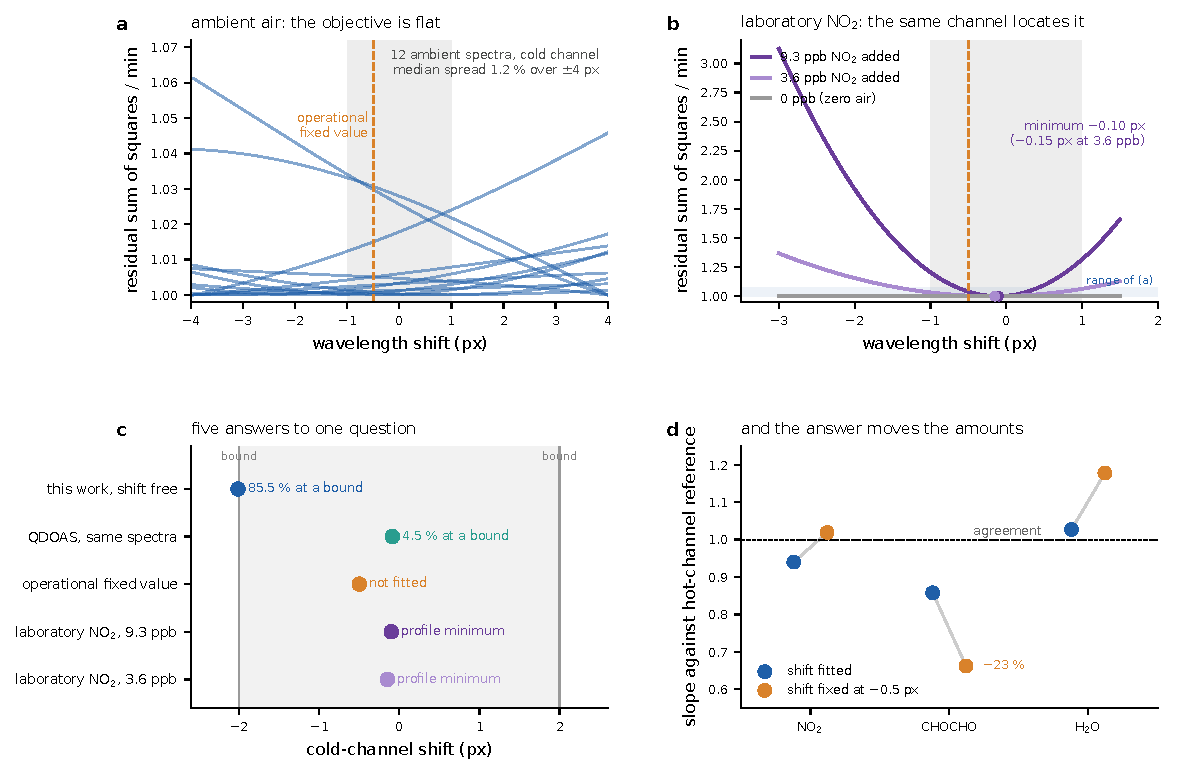
\includegraphics[width=\textwidth]{figures/fig05.pdf}
\caption{Identifiability of the cold-channel wavelength shift. \textbf{(a)} Profiled residual sum of squares against
shift for twelve ambient spectra, each normalised to its minimum; shaded, the range the operational configuration
allows; dashed, the value it fixes. \textbf{(b)} The same scan for the laboratory spectra of 2 June (zero air with 9.3
and 3.6\,ppb NO$_2$ added, and zero air alone); band, the vertical range of (a). \textbf{(c)} Shift returned for the
ambient spectra by two implementations under matched settings (with the fraction of fits at a bound), the operational
fixed value and the profile minima of (b). \textbf{(d)} Regression slope between the cold-channel retrievals of Augur
and QDOAS on the same spectra ($n = \fieldnum{5364}$), with Augur's shift fitted and fixed.}
\label{fig:5}
\end{figure*}

The budget of Sect.~\ref{sec:4} is not an artefact of basin hopping in the shift, and the reflectivity term hardly couples to
the shift at all (Appendix~\ref{app:D}, Table~\ref{tab:shift_degeneracy}).

Reporting \fieldnum{$-2.014 \pm 0.03$}\,px for a quantity the data locate only to \fieldnum{$\pm 2$}\,px is the failure described here, and
for this channel the resulting term is larger than any in Table~\ref{tab:2}. The ratio of the objective at the returned
value to that at a fixed reference point, which the fit evaluates anyway, would flag it (Sect.~\ref{sec:6.1}). Because
the shift belongs to the spectrograph rather than to the air, it could also be fitted jointly across the spectra of a
calibration block, as a separable problem with common nonlinear parameters. This is not implemented here and would
need an absorber in the block, as in the laboratory spectrum of Fig.~\ref{fig:5}b.

\subsection{Termination at a bound is a routine outcome}
\label{sec:5.2}

In this instrument bound termination is the normal state of one channel and a systematic response to perturbation in
another. The operational configuration (Appendix~\ref{app:A}) bounds the shift to $[-10, +0.5]$\,px in hot ANs and
$[-5, +5]$\,px in hot PNs and fixes it at $-0.5$\,px in the cold channel. In a sensitivity run that instead bounded the
cold shift to $[-1, +1]$\,px, every one of the \fieldnum{22} base fits returned exactly \fieldnum{$-1.000$}\,px, the bound itself, and was
reported as converged. In the production propagation of Sect.~\ref{sec:4} the cold shift is held fixed, as in operation,
and moves by exactly zero in every record, which confirms the configuration but also means the channel contributes
no information about the parameter.

On the clock-aligned basis of Table~\ref{tab:2}, \fieldnum{187} of the \fieldnum{9034} $\Sigma$ANs records are excluded because a fit of
either channel, unperturbed or perturbed, terminated at a bound. The split by perturbation was recorded only for the
earlier run on the unaligned reference: there, in hot PNs, the zero-air perturbation accounted for \fieldnum{121}
bound-terminated records against \fieldnum{4} for the unperturbed fits (the categories overlap), and the hot ANs channel had
none. In that run the operational fit was well inside its feasible region and the structural perturbation drove it
out, so the margin between the operational solution and the edge of identifiability is smaller than the size of a
reference error. Augur computes the termination states internally; the delivered campaign product did not carry them,
and the current version exports them as separate columns (Sects.~\ref{sec:2.6} and \ref{sec:6.1}).

\subsection{How far a record is from its calibration}
\label{sec:5.3}

The distance in time from a record to the calibration knots that produced its references varies over the campaign by
more than an order of magnitude, and the pipeline computes it in order to interpolate and then discards it. The
retrieval interpolates the reflectivity across an \fieldnum{11.8}\,h gap exactly as across a one-hour gap and returns the same
uncertainty in both cases. Coverage was measured over the whole campaign from calibration blocks extracted directly from the raw files,
independently of the retrieval. The extraction reproduces the production knot cache (\fieldnum{157}/\fieldnum{157} hot and
\fieldnum{164}/\fieldnum{164} cold knots at 0.000000\,s) and the alpha header's own \texttt{ZA\_count=}\fieldnum{1313}. Two distinct
deficits appear: records outside the knot range, and records inside a knot gap longer than two hours
(Table~\ref{tab:coverage}).

\begin{table}[t]
\caption{Calibration coverage of the retrieved records, from calibration blocks extracted directly from the raw files: number of records $n$; percentage of records outside the knot range and inside a knot gap longer than 2\,h (counts from the coverage
extractor; the retrieval itself has \fieldnum{9149} ambient records per heated channel in the budget window), for the zero-air ($I_0$) and reflectivity ($R$) references; and the longest reflectivity gap.}
\label{tab:coverage}
\small\setlength{\tabcolsep}{3pt}
\begin{tabular}{llllllll}
\tophline
instrument & window & $n$ & $I_0$ out of range & $I_0$ gap $>2$\,h & $R$ out of range & $R$ gap $>2$\,h & worst $R$ gap \\
\middlehline
hot ch1/ch2 & campaign & \fieldnum{76\,282} & \fieldnum{0.08}\,\% & \fieldnum{0.07}\,\% & \fieldnum{3.76}\,\% & \fieldnum{1.23}\,\% & \fieldnum{10.6}\,h \\
hot ch1/ch2 & budget window 05-18..24 & \fieldnum{9\,088} & \fieldnum{0.01}\,\% & \fieldnum{0.00}\,\% & \fieldnum{0.00}\,\% & \fieldnum{0.00}\,\% & \fieldnum{1.3}\,h \\
cold & campaign & \fieldnum{43\,259} & \fieldnum{0.13}\,\% & \fieldnum{0.34}\,\% & \fieldnum{2.89}\,\% & \fieldnum{11.03}\,\% & \fieldnum{11.8}\,h \\
cold & cold window 06-10..16 & \fieldnum{7\,069} & \fieldnum{0.42}\,\% & \fieldnum{0.00}\,\% & \fieldnum{17.32}\,\% & \fieldnum{18.31}\,\% & \fieldnum{11.8}\,h \\
\bottomhline
\end{tabular}
\end{table}

For the zero-air reference the interpolation is genuine: \fieldnum{0.08}\,\% of hot records lie outside the knot range and
\fieldnum{0.07}\,\% inside a gap longer than two hours, with the nearest knot a median \fieldnum{922}\,s away. The zero-air knot set is on
the corrected time axis -- the production cache over 05-18..24 reproduces a re-extraction at 0.000000\,s -- so the
$I_0$ column is unaffected by the displacement of Sect.~\ref{sec:5.4}.

The cold channel's deficit is a gap problem. The existing quality gates reject \fieldnum{11.3}\,\% of cold pairs against
\fieldnum{0.24}\,\% of hot pairs (\fieldnum{3} of \fieldnum{1\,264}); an independent count gives \fieldnum{75} of \fieldnum{743}, \fieldnum{10.1}\,\%, and nothing below turns on
the difference. Independent rejection at the \fieldnum{11.3}\,\% rate would leave \fieldnum{3.5}\,\% of cold records in gaps longer than two
hours, against the \fieldnum{11.03}\,\% observed. The worst gap, \fieldnum{11.8}\,h, is eleven consecutive rejected pairs, a run expected
0.03 times in the campaign even at a 40\,\% independent rejection rate. The rejections arrive in runs,
the episodic structure that Sect.~\ref{sec:6.1a} finds in the reflectivity variance itself. The same failures are absent
from the budget population (Sect.~\ref{sec:4.4}). In the cold channel, eleven of the thirteen zero-air blocks
identified as defective in Sect.~\ref{sec:6.3} fall outside the case set, because no reflectivity knot exists within
\fieldnum{2.8}--\fieldnum{5.8}\,h of them. A collapse of the zero-air signal takes the He/zero-air pair down with it, so
the two reference failures are one event seen twice. The interpolation already holds the time to the nearest knot, the length of the enclosing interval and whether a
record is out of range. Reported, they would separate the \fieldnum{0.00}\,\% of the budget window from the \fieldnum{18.31}\,\% of the cold
window, which no field in the current product distinguishes (Sect.~\ref{sec:6.1}).

\subsection{A reference error the fit does not see}
\label{sec:5.4}

The operational reflectivity reference was not clock-aligned. Its knots for 2026-05-18 to 05-30 lie on a time axis
that a later correction to the raw-data reader superseded, while the spectra lie on the corrected one. Every record in
that span, including the budget window of Sect.~\ref{sec:4}, was therefore retrieved with a reflectivity displaced by
nine hours. The zero-air reference is unaffected, because its knots were already on the corrected axis (verified to
0.000000\,s), and so is the cold channel, to which the correction does not apply. The retrieval was run twice over all
\fieldnum{9\,132} records of the window common to both heated channels, changing nothing but the knot time base
(Table~\ref{tab:clock_displacement}).

\begin{table}[t]
\caption{Change in the retrieved amounts when the heated channels are retrieved with the clock-aligned instead of the nine-hour-displaced reflectivity knots, over the records of the budget window: robust scale (rSD) and standard deviation (SD) of the change (ppb), and the rSD of the change relative to the rSD of the $R$ term in Table~\ref{tab:2}. $\Sigma$ANs is formed with $g' = \fieldnum{0.9524}$ as in Table~\ref{tab:2}.}
\label{tab:clock_displacement}
\begin{tabular}{llll}
\tophline
series & delta rSD (ppb) & delta SD (ppb) & vs the $R$ term of Table~\ref{tab:2} \\
\middlehline
ANs channel & \fieldnum{0.1048} & \fieldnum{0.1627} & \fieldnum{3.0} \\
PNs channel & \fieldnum{0.0358} & \fieldnum{0.0563} & \fieldnum{2.8} \\
$\Sigma$ANs & \fieldnum{0.100} & \fieldnum{0.1418} & \fieldnum{3.7} \\
\bottomhline
\end{tabular}
\end{table}

The displacement moves the alkyl nitrate product by \fieldnum{0.100}\,ppb, between three and four times the reflectivity term of
the budget and \fieldnum{1.44} times the whole of it. It is the largest term we can quantify within the retrieval; the
multiplicative scale discrepancy of Sect.~\ref{sec:3.6} is larger but lies outside it. It is not in Table~\ref{tab:2},
which measures what a reference's own uncertainty costs rather than what using the wrong reference costs.

\begin{table}[t]
\caption{What the fit report shows for the displacement of Table~\ref{tab:clock_displacement}: RMS change of the extinction spectrum (cm$^{-1}$), ratio of the residual and of the reported $\sigma$ between the two retrievals, change in the retrieved amount in units of the reported $\sigma$, and change in the fitted shift.}
\label{tab:clock_fitreport}
\begin{tabular}{llllll}
\tophline
 & $\alpha$ RMS change & residual ratio & reported $\sigma$ ratio & $|\delta c| / \sigma$ & $|\delta\,\mathrm{shift}|$ \\
\middlehline
ANs & $\fieldnum{3.37\times10^{-9}}$ & \fieldnum{1.0020} & \fieldnum{1.0022} & \fieldnum{1.99} & \fieldnum{0.0053}\,px \\
PNs & $\fieldnum{1.53\times10^{-8}}$ & \fieldnum{1.0016} & \fieldnum{1.0016} & \fieldnum{0.55} & \fieldnum{0.0065}\,px \\
\bottomhline
\end{tabular}
\end{table}

The fit report does not register the displacement (Table~\ref{tab:clock_fitreport}). The extinction spectrum changes by
an amount comparable to the single-scan noise floor of $\fieldnum{6.16\times10^{-9}}$, and the residual and the reported
uncertainty change by the same two parts in a thousand. The agreement is expected, because the reported uncertainty is a near-constant multiple of the residual RMS
(Sect.~\ref{sec:7.3}); an unchanged residual and an unchanged uncertainty are one witness reported twice. The fitted wavelength shift moves by \fieldnum{0.005}\,px, where the reference perturbations of
Table~\ref{tab:2} move it by \fieldnum{0.243}\,px (median), about forty times more, so the error is neither absorbed by the
nonlinear parameters nor revealed by the residual. The retrieved concentration of the 300\,$^{\circ}$C channel moves by two
reported standard deviations while every quality indicator in the fit report stays the same.

Correcting the time base changed the budget in both directions. The robust scale of the $\Sigma$ANs budget fell by
\fieldnum{7.0}\,\% (\fieldnum{0.0745} to \fieldnum{0.0693}\,ppb) while its standard deviation rose by \fieldnum{4.5}\,\% (\fieldnum{0.1183} to \fieldnum{0.1236}). The total
uncertainty relative to what is reported therefore widened at both ends, from \fieldnum{1.70}--\fieldnum{2.41} to \fieldnum{1.63}--\fieldnum{2.50}
times the same fit-reported sigma (Sect.~\ref{sec:4.4}). Coverage improved, from \fieldnum{8505} to \fieldnum{9034} of the window's \fieldnum{9149}
ambient records (\fieldnum{93.0} to \fieldnum{98.7}\,\%), because the misaligned knots had been falling outside the one-hour window that
admits a record to the perturbation experiment. The correlation between the two channels' joint responses fell from
\fieldnum{$+0.412$} to \fieldnum{$+0.146$}: because $\Sigma$ANs is a channel difference, a common-mode error partly cancels in it, and the
pre-correction cancellation was an artefact of an error the two channels shared. Both effects were properties of the
contaminated product, and the budget measured on it inherited them.

The cost of the displacement depends on how fast the reflectivity was moving. Across the boundary where the clock was
corrected, the affected side gives \fieldnum{0.0622}\,ppb against \fieldnum{0.0000}\,ppb on the unaffected side, which confirms that the
realignment touched only the intended knots. The displacement thus costs less near the boundary than in the budget
window, where the reflectivity moved fastest. The budget-window figure of \fieldnum{0.100}\,ppb is the value to quote;
\fieldnum{0.0622}\,ppb is range information, not a worst case.

The underlying cause was a stale derived file. The heated-channel clock itself ran on local time until 29 May and was
corrected in the reader after comparison with an external time reference. The reflectivity file was
written on 2026-07-10, the correction that invalidated it was committed on 2026-09-19, and the retrieval read both
without comparing them. Recording, for each derived reference, the version of the code and the raw files it was built
from detects this condition mechanically (Sect.~\ref{sec:6.1}); it is the only failure in this paper that admits a
complete remedy rather than a better report.
